% ----------------------------------------------------
% DAB Processing
% ----------------------------------------------------
\documentclass[class=report,11pt,crop=false]{standalone}
\input{../Style/ChapterStyle.tex}
\makenoidxglossaries

\newacronym{radar}{RADAR}{Radio Detection and Ranging}
\newacronym{dab}{DAB}{Digital Audio Broadcasting}
\newacronym{fm}{FM}{Frequency Modulation}
\newacronym{am}{AM}{Amplitude Modulation}
\newacronym{fdm}{FDM}{Frequency Division Multiplexing}
\newacronym{ofdm}{OFDM}{Orthogonal Frequency Division Multiplexing}
\newacronym{cofdm}{COFDM}{Coded Orthogonal Frequency Division Multiplexing}
\newacronym{dvbt2}{DVB–T2}{Digital Video Broadcasting — Second Generation Terrestrial}
\newacronym{em}{EM}{electromagnetic}
\newacronym{icasa}{ICASA}{Independent Communications Authority of South Africa}
\newacronym{ioo}{IOO}{Illuminators of Opportunity}
\newacronym{pr}{PR}{Passive Radar}
\newacronym{qpsk}{QPSK}{Quadrature Phase-Shift Keying}
\newacronym{dqpsk}{DQPSK}{Differential~Quadrature~Phase-Shift~Keying}
\newacronym{etsi}{ETSI}{European Telecommunications Standards Institute}
\newacronym{psk}{PSK}{Phase Shift Keying}
\newacronym{ask}{ASK}{Amplitude-Shift Keying}
\newacronym{fsk}{FSK}{Frequency-Shift Keying}
\newacronym{iq}{IQ}{In-phase and Quadrature}
\newacronym{ns}{NS}{Null Symbol}
\newacronym{prs}{PRS}{Phase Reference Symbol}
\newacronym{fic}{FIC}{Fast Information Channel}
\newacronym{msc}{MSC}{Main Service Channel}
\newacronym{dft}{DFT}{Discrete Fourier Transform}
\newacronym{idft}{IDFT}{Inverse Discrete Fourier Transform}
\newacronym{fft}{FFT}{Fast Fourier Transform}
\newacronym{ifft}{IFFT}{Inverse Fast Fourier Transform}
\newacronym{fec}{FEC}{Forward Error Correction}
\newacronym{ard}{ARD}{Amplitude-Range-Doppler}
\newacronym{snr}{SNR}{Signal-to-Noise Ratio}
\newacronym{isi}{ISI}{Intersymbol Interference}
\newacronym{mcm}{MCM}{Multicarrier Modulation}
\begin{document}
% ----------------------------------------------------
\chapter{Digital Audio Broadcasting: Processing}
\epigraph{Nobody can build you the bridge over which you must cross the river of life, nobody but you alone.}%
    {\emph{Friedrich Nietzsche}}
% ----------------------------------------------------

\section{Overview}

\begin{figure}[htbp]
    \centering
    \includegraphics[width=\linewidth]{BD_Overview_All.pdf}
    \caption{Block diagram showing entire DAB processing chain}
    \label{fig:BD_Overview_All}
\end{figure}

\section{Pre-processing}
\subsection{Reading IQ data from file}
\subsection{Resampling IQ data}
\subsection{Frame Synchronization via Phase Reference Symbol}
\subsection{Frame Extraction}

\section{Demodulation}
\subsection{Overview}

\begin{figure}[htbp]
    \centering
    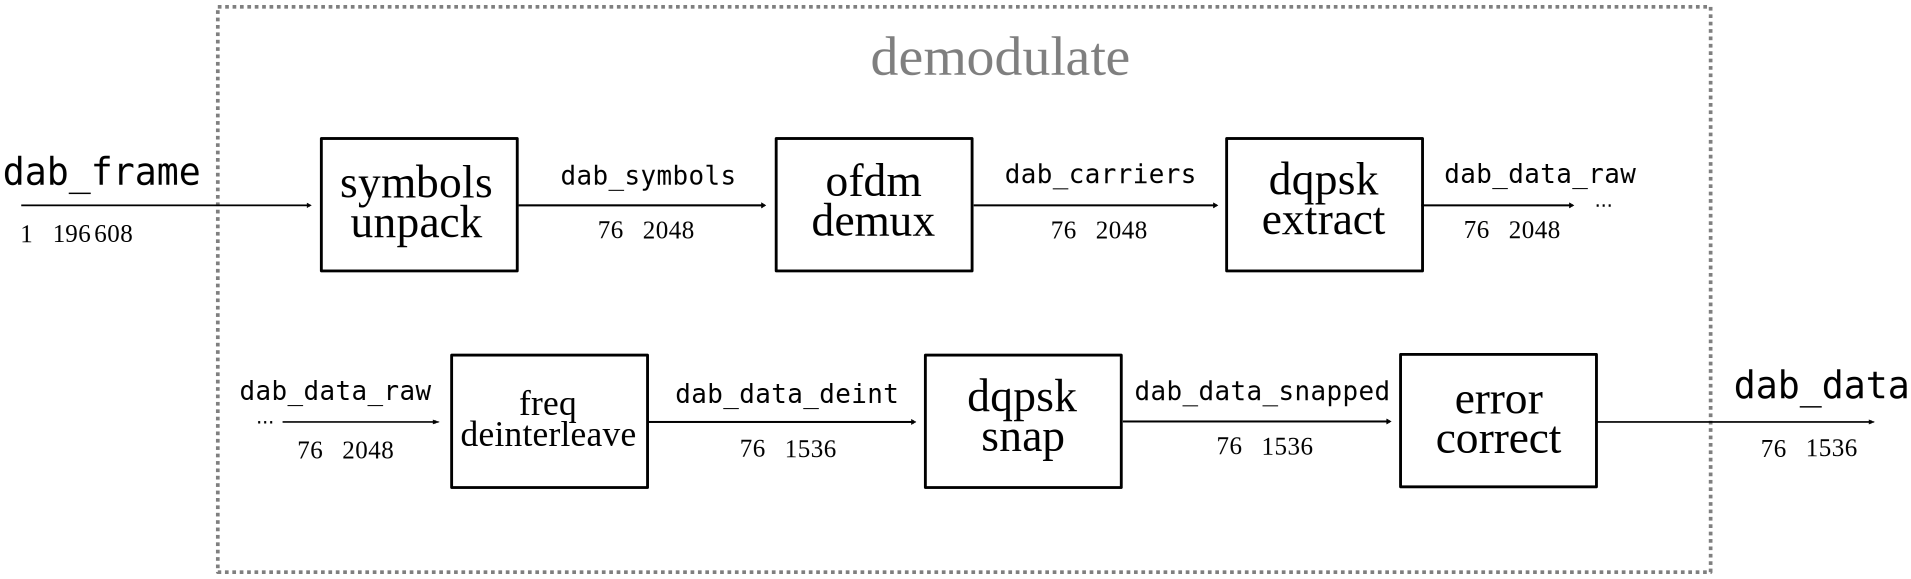
\includegraphics[width=\linewidth]{BD_Demod_All.pdf}
    \caption{Block diagram showing entire DAB demodulation processing chain}
    \label{fig:BD_Demod_All}
\end{figure}

\subsection{Block Unpacking}
\subsection{OFDM Demultiplexing}
\subsection{DQPSK Extraction}
\subsection{Frequency Deinterleaving}
\subsection{DQPSK Snapping}
\subsection{Error Correction}

\section{Re-modulation}
\subsection{Overview}
\subsection{Frequency Interleaving}
\subsection{DQPSK Building}
\subsection{OFDM Multiplexing}
\subsection{Block Packing}

\section{Summary}

% ----------------------------------------------------
\ifstandalone
\bibliography{../Bibliography/References.bib}
\printnoidxglossary[type=\acronymtype,nonumberlist]
\fi
\end{document}
% ----------------------------------------------------